\chapter{\Vauc as a toolkit}

\Vauc provides several programs that manipulate various type of
automata. In this chapter we will learn
how to use those programs. Actually there are 6 programs
located in src/demos/function\_library/ directory. Each of them
dealing with a specific type of automata:


\begin{itemize}
  \item b for manipulating automata over Boolean semiring $\mathbb{B}$;
  \item z for manipulating automata over $(\mathbb{Z},+)$;
  \item z\_min\_plus for manipulating automata over $(\mathbb{Z},min)$;
  \item z\_max\_plus for manipulating automata over $(\mathbb{Z},max)$;
  \item rt\_tdc for manipulating realtime transducers;
  \item tdc for manipulating automata over free monoid product.
\end{itemize}


%%Example on boolean automaton
\section{Boolean automata}

\subsection{A first example}

Let's consider the following boolean automaton :

%%Schema de l'automate A
\begin{figure}[ht] \centering
  \begin{VCPicture}{(0,-2)(6,2)}
    % states
    \State{(0,0)}{A} \State{(3,0)}{B} \State{(6,0)}{C}
    % initial--final
    \Initial{A} \Final{C}
    % transitions
    \EdgeL{A}{B}{a} \EdgeL{B}{C}{b}
    \LoopS[.5]{A}{b} \LoopN[.5]{A}{a} \LoopS[.5]{C}{b} \LoopN[.5]{C}{a}
    %
  \end{VCPicture}
  \caption{The automaton $A_1$}
\end{figure}

You can find the XML code that describe this automaton in
doc/manual/examples/a1.xml.
We will use \Vauc to compute the determinized automaton of $A_1$ and
then we will minimize the resulting automaton.

\subsubsection{Determinization of $A_1$}
Computing the determinized of a boolean automaton is simply realized
by calling \textit{determinize} function :
\begin{alltt}
# ./b determinize a1.xml > a1\_det.xml
\end{alltt}
Now the file a1\_det.xml contains the XML description of the
determinized of the automaton A.

\subsubsection{Visualizing}

We can get some information about our newly created automaton by calling
the \textit{info} function:
\begin{alltt}
# ./b info a1\_det.xml
\textit{States: 4
Transitions: 8
Initial states: 1
Final states: 2}
\end{alltt}
Or we can use dotty to visualize our newly created automaton:
\begin{alltt}
# ./b display a1\_det.xml
\end{alltt}

%%Dotty output of det(A1)
\begin{figure}[ht]
  \centering
  \scalebox{0.7}{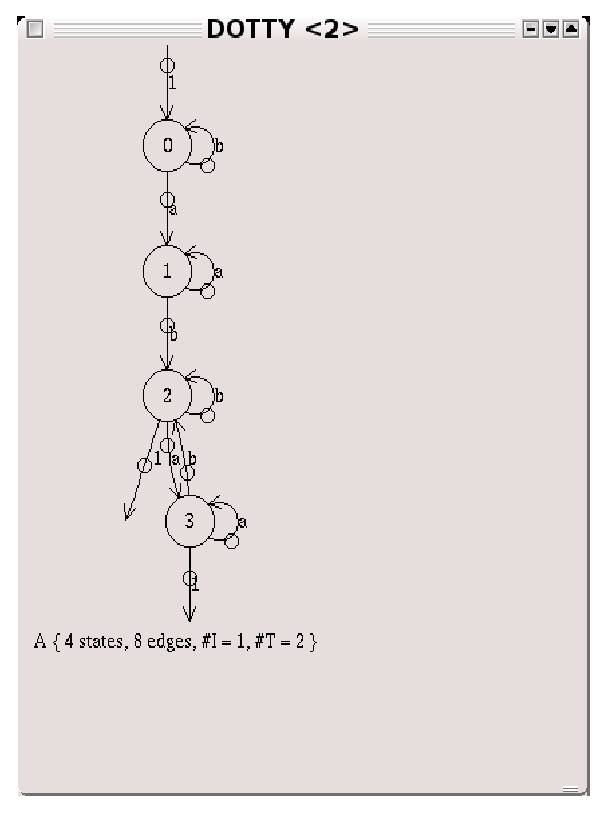
\includegraphics{images/a1_det.eps}}
  \caption{Determinized of $A_1$}
\end{figure}

\subsubsection{Minimizing}

\begin{alltt}
# ./b determinize a1.xml | ./b minimize - | ./b display -
\end{alltt}

%% Dotty min(det(A1))
\begin{figure}[!ht]
  \centering
  \scalebox{0.7}{\includegraphics{images/a1_det_min.eps}}
  \caption{Minimizing the Determinized of $A_1$}
\end{figure}

\subsubsection{Evaluation}

Evaluating if a word is accepted by our automaton :
\begin{alltt}
# ./b eval a1.xml 'abab'
\textit{1}
# ./b eval a1.xml 'bbba'
\textit{0}
\end{alltt}
where 1 (resp. 0) means that the word is accepted (resp. not accepted)
by the automaton.

\subsection{Rationnal expressions and boolean automata}

\Vauc provides functions for manipulating rationnal expressions
associated to boolean automata. For instance, computing the language
recognized by a boolean automaton can be done thanks to the
\textit{aut\_to\_exp} function:
\begin{alltt}
# ./b aut_to_exp a1.xml
\textit{(a+b)*.a.b.(a+b)*}
# ./b aut_to_exp a1_det.xml
\textit{b*.a.a*.b.(a.a*.b+b)*.(a.a*+1)}
\end{alltt}
Plus \Vauc provides several algorithms that build an automaton that
recognizes a given language. For instance let's build the standard
automaton that recognizes the language "$(a+b)*a.b.(a+b)*$" and
minimize the resulting automaton:

\begin{alltt}
# /b standard_of "(a+b)*a.b.(a+b)*" | ./b minimize - | ./b display -
\end{alltt}
\begin{figure}[ht]
  \centering
  \scalebox{0.7}{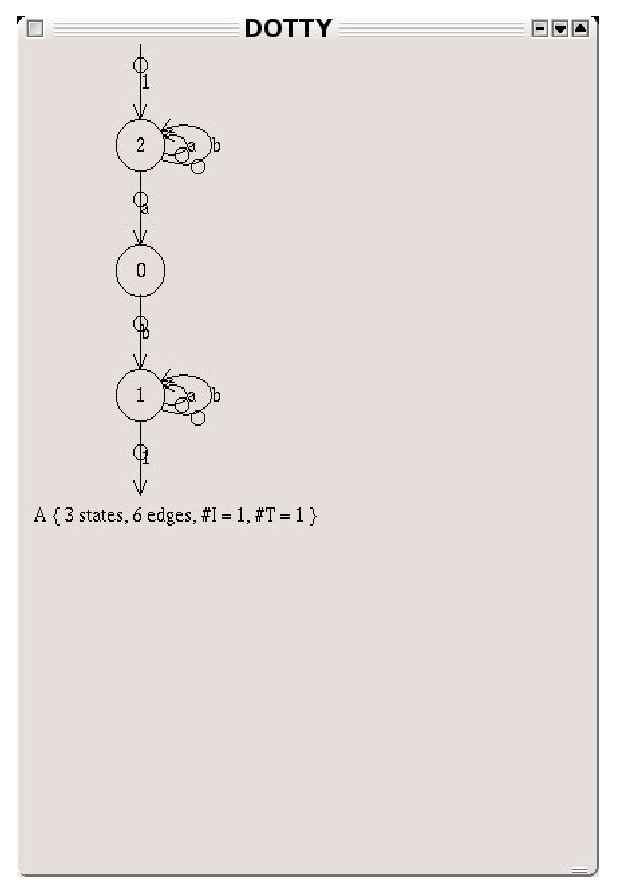
\includegraphics{images/a1.eps}}
  \caption{The minimize standard automaton of "(a+b)*a.b.(a+b)*"}
\end{figure}
Please note that your rationnal expressions should follow the
following grammar :
\begin{verbatim}
         exp ::= '(' exp ')'
         |   exp '+' exp
         |   exp '.' exp
         |   exp exp
         |   exp '*'
         |   weight ' ' exp
         |   exp ' ' weight
         |   0
         |   1
         |   word
\end{verbatim}

\subsection{Building your own automaton}
%%FIXME: Here we should give a small example of define_automaton
%%function.

\section{Transducers}
\subsection{Example}

\section{Weighted automata}
\subsection{Example}

\section{List of available functions}

\begin{itemize}
  \item is-empty
  \item are-isomorphic
  \item accessible
  \item coaccessible
  \item realtime
  \item trim
  \item transpose
  \item aut\_to\_exp
  \item expand
  \item standard\_of
  \item thompson\_of
  \item derived\_terms
  \item product
  \item power
  \item determinize
  \item minimize
  \item quotient
  \item closure
  \item eval
  \item display
  \item info
\end{itemize}
